\chapter{Logica proposizionale}

\section*{Sintassi e semantica}
Prima di passare alla logica proposizionale, dobbiamo fare una distinzione tra sintassi e semantica.

La \textbf{sintassi} riguarda il modo di scrivere attravarso un linguaggio da noi definito. Serve per costruire oggetti, o per verificare se gli oggetti costruiti sono sintatticamente corretti oppure no.

La \textbf{semantica} rappresenta tutto quello che riguarda il significato di ciò che scriviamo.

Possiamo vedere un'espressione aritmetica come o un numero o come l'operazione che si svolge tra altre due espressioni:
\begin{center}
    Exp::=N$|$(Exp op Exp)
\end{center}
E' vero perchè è dimostrabile per induzione.
Caso base: Numero ::= n;
Passo induttivo: è possibile perchè N::=0$|$(Succ.N) (o zero o una successione di un numero).

Ad esempio possiamo chiederci quando $((3*7)-2)+(12-4)$ è sintatticamente corretta?

L'equazione è sintatticamente corretta quando tutte le parti composte dell'equazione, sono a loro volta delle equazioni.

\section{Connettivi logici}
Il linguaggio della logica proposizionale è formato da un'insieme di simboli (in genere le prime lettere maiuscole dell'alfabeto) e da connettivi che hanno lo stesso ruolo degli operatori aritmetici.

\begin{table}[ht]
    \centering
    \begin{tabular}{|cc|c|c|c|c|c|}
        \hline S & Simboli & A & B & C & $A_1$ & $A_2$\\\hline
        C & Connettivi & $\neg$ & $\land$ & $\lor$ & $\Longrightarrow$ & $\iff$\\
        && NOT & AND & OR & IMPLICA & SE E SOLO SE\\\hline
    \end{tabular}
    \caption{Linguaggio della logica proposizionale}
    \label{tab:lp_tab}
\end{table}

Notiamo come solo il not accetta solo un argomento, tutti gli altri ne devono avere due. Infatti si può fare una prima distinzione tra operatori unari e binari.

\section{Classificazione delle formule proposizionali}
Passiamo ora alla classificazione delle formule proposizionali. Una formula si definisce:
\begin{itemize}
    \item \textbf{Soddisfacibile} se esiste un'assegnamento di verità (V o F) che la rende vera.
    \item \textbf{Insoddisfacibile} se non esiste un'assegnamento di verità (V o F) che la rende vera (es. $A\land\neg A$).
    \item \textbf{Falsificabile} se esiste un'assegnamento di verità (V o F) che la rende falsa.
    \item \textbf{Valido o tautologico} se ogni assegnamento di verità (V o F) la rende vera (es. $A\lor\neg A$).
    \item \textbf{Conseguenza logica} diremo inoltre che F è
conseguenza logica di G quando F vale in tutti i modelli in cui valgono tutte le formule di G. E si esprime scrivendo $G\models F$.
\end{itemize}

\section{Tableau proposizonali}
Il metodo dei tableau proposizionali è originariamente un procedimento per provare la soddisfacibilità di un enunciato. Esso, infatti, decompone l’enunciato fino alle sue componenti elementari.

I tableau proposizionali sono grafi ad albero costituiti da una disposizione piana di nodi, contenenti uno o più enunciati; il primo nodo (detto radice dell’albero) contiene sempre l’enunciato in esame. A partire da questo viene costruita, attraverso regole di eliminazione dei connettivi, una tabella ramificata con nodi etichettati da enunciati sempre meno complessi, fino a giungere ai singoli enunciati componenti o i loro negati.

La costruzione ha termine quando tutti gli ultimi nodi dei rami contengono solamente enunciati atomici o loro negazioni.
Pertanto, se all’ultimo nodo di un ramo appartengono contemporaneamente un enunciato A e la sua negazione $\neg$A, si dice che il ramo è chiuso; quando tutti i rami sono chiusi, il tableau è chiuso e la confutazione è completata, perchè esclude ogni soddisfacibilità.

Consideriamo ora in generale i connettivi $\land$ e $\lor$: in quale caso possiamo dire che X $\land$ Y è vero? Occorre che ambedue gli enunciati X e Y siano veri. In quale caso, invece, possiamo dire che X $\lor$ Y è vero? Se e solo se almeno uno tra X ed Y è vero. Dunque nel caso di X $\lor$ Y dobbiamo creare una biforcazione del grafo, su uno dei due nodi generati porre X e sull’altro Y, perchè si vengono a creare due situazioni, ugualmente accettabili per i nostri scopi.

\subsection*{Regole}

\textbf{Regola($\alpha$1):}
\begin{gather*}
    X \land Y\\
    |\\
    X, Y
\end{gather*}
\textbf{Regola($\alpha$2):}
\begin{gather*}
    \neg(X \lor Y)\\
    |\\
    \neg X, \neg Y
\end{gather*}
\textbf{Regola($\alpha$3):}
\begin{gather*}
    \neg(X \implies Y)\\
|\\
X, \neg Y
\end{gather*}
\textbf{Regola($\alpha$4):}
\begin{gather*}
    X \iff Y\\
|\\
X \implies Y, Y \implies X
\end{gather*}
\textbf{Regola($\alpha$5):}
\begin{gather*}
    \neg\neg X\\
|\\
X
\end{gather*}
\textbf{Regola($\beta$1):}
\begin{gather*}
    X \lor Y\\
/\backslash\\
X\hspace{0,5cm}Y
\end{gather*}
\textbf{Regola($\beta$2):}
\begin{gather*}
    \neg(X \land Y)\\
/ \backslash\\
\neg X\hspace{0,5cm}\neg Y
\end{gather*}
\textbf{Regola($\beta$3):}
\begin{gather*}
    X \implies Y\\
/ \backslash\\
\neg X\hspace{0,5cm}Y
\end{gather*}
\textbf{Regola($\beta$4):}
\begin{gather*}
    \neg(X \iff Y)\\
/ \backslash\\
\neg(X \implies Y)\hspace{0,5cm} \neg(Y \implies X)
\end{gather*}

\begin{example}\label{es_prop1}
Confutiamo $\neg(((A \implies B) \land (B \implies C)) \implies (A \implies C))$.
Applichiamo innanzitutto la regola ($\alpha$3) e otteniamo:
\begin{gather*}
\neg(((A \implies B) \land (B \implies C)) \implies (A \implies C))\\
|\\
(A \implies B) \land (B \implies C), \neg(A \implies C)
\end{gather*}
Applichiamo la regola ($\alpha$1) al primo dei due enunciati ottenuti:
\begin{gather*}
(A \implies B) \land (B \implies C), \neg(A \implies C)\\
|\\
A \implies B, B \implies C, \neg(A \implies C)
\end{gather*}
e quindi la regola ($\alpha$3) all’enunciato $\neg(A\implies C)$:
\begin{gather*}
A \implies B, B \implies C, \neg(A \implies C)\\
|\\
A \implies B, B \implies C, A, \neg C
\end{gather*}
Applichiamo le regole $\beta$ ottenendo il seguente risultato:
\begin{figure}[ht]
    \centering
    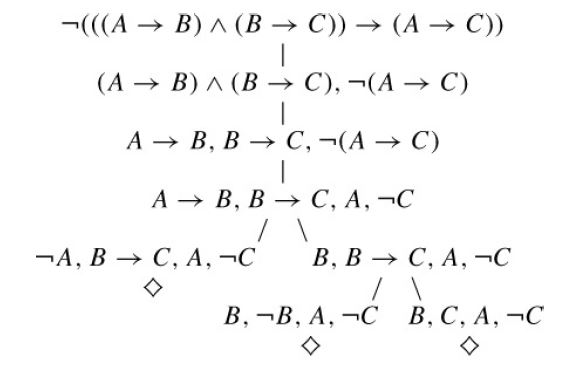
\includegraphics[width = 8cm]{images/proposizioni_es1.JPG}
    \caption{Risultato finale dell'esercizio \ref{es_prop1}}
\end{figure}

Il ramo di sinistra è chiuso, in quanto nell’ultimo nodo troviamo sia A che $\neg A$.
I due rami a destra, invece, sono entrambi chiusi: quello a sinistra per la presenza contemporanea di $\neg B$ e B nell’ultimo nodo; quello a destra per la presenza contemporanea di C e $\neg C$ nell’ultimo nodo.

Tutti i rami del tableau risultano dunque chiusi: l’enunciato di partenza è confutato e ciò significa che la sua negazione, cioè $((A \implies B) \land (B \implies C)) \implies (A \implies C)$, è una tautologia.
\end{example}